\chapterimage{chapter_head_1.png}

\chapter{Objekterkennung und Computer Vision}
\section{Intro \& Motivation}
Wie können wir uns eigentlich in der Welt, in der wir sind, zurechtfinden? Die \textbf{Wahrnehmung} ermöglicht die Aufnahme von Informationen über die Umgebung. Der Menschen hat fünf Hauptwahrnehmungssinne: Sehen, Hören, Tasten, Riechen und Schmecken. Können wir einer künstlichen Intelligenz (KI) diese Wahrnehmung beibringen? Wenn ja, wie?

Sinne bei KIs nennen wir \textbf{Sensoren}. Solche, die wir in KIs einbauen können, sind Sehen, Hören und Tasten. \textbf{Sehen} ist dabei im Hinblick auf den Gebrauch von KIs in der physischen Welt für uns Menschen der hilfreichste von allen.

In dieser Ausarbeitung werden zunächste Grundlagen über die Funktionsweise des Sehens beschrieben. Der Fokus wird dann auf die Verarbeitung von gewonnenen Rohinformationen liegen und ein paar Anwendungen ansprechen.

\section{Überblick Computer Vision}
Die Frage die Computer Vision stellt, ist eigentlich recht einfach: Wenn ein von der Umgebung ausgelöster Sensor-Impuls (S) so und so aussieht, wie sieht dann die Umgebung (W) dazu aus? Leider ist das Invertieren dieser Funktion
\begin{equation*}
S = f(W) \Rightarrow W = f^{-1}(S)
\end{equation*}
nicht so einfach möglich. Man muss sich also überlegen, anhand welcher Merkmale Entscheidungen über den Inhalt eines Bildes getroffen werden können. Computer Vision lässt sich dafür grob in drei Stufen einteilen:
\begin{itemize}
\item \textit{Low-Level Vision}: Grundlegende Untersuchung des Bildes auf herausstechende Features wie Unterschiede in Helligkeit, Farben oder Texturen und die damit verbundene Kantendetektion
\item \textit{Medium-Level Vision}: Objekterkennung und Bewegungsanalyse mithilfe der zuvor gesammelten Informationen
\item \textit{High-Level Vision}: Die Kombination und Analyse aller Daten: Was sagt mir das Bild, wie reagiere ich darauf?
\end{itemize}

Die Hauptanwendungsgebiete hierfür sind:
\begin{itemize}
\item Manipulation: Die Erlangung von benötigen Informationen von und Rückmeldung über lokale Gebilde, um mit diesen zu interagieren (z.~B.\ greifen, einfügen; Anwendung: z.~B.\ Qualitätskontrolle).
\item Navigation: Die Berechnung der eigenen Geschwindigkeit und Position (Ausrichtung), um Routen zu planen und Hindernissen auszuweichen.
\item Objekterkennung: Die Charakterisierung von Objekten zur Unterscheidung von \glqq gut\grqq\ und \glqq schlecht\grqq\ (z.~B.\ Beute- und Raubtier, (un)genie"sbare Früchte, Bekannte und Fremde).
\end{itemize}

Wir werden uns hier nur mit Low-Level- und Medium-Level Vision beschäftigen.
Zunächst werden wir auf die Entstehung von Bildern, Bildverarbeitungsoperationen, nutzbare Hinweise in Bildern, optisch gesteuerte Manipulation und Navigation und schließlich verschiedene Ansätze zur Objekterkennung eingehen.

\subsection{Grundlagen der Bildentstehung}

Um Informationen über einen \textbf{Ort} zu erhalten, benötigen wir ein Bild. Um ein \textbf{Bild} (2D) zu erstellen, müssen wir \textbf{Sehen} (3D) können. Das Sehen, so wie es in unseren Augen passiert, ist sehr komplex. Vereinfacht können wir es jedoch  anhand einer Lochkamera erkl"aren - der Prozess ist ungef"ahr der Gleiche.

\subsubsection{Lochkamera}

\marginpar[Links]{\small{(wer mit diesem Prinzip bereits vertraut ist, kann die nächste Seite überspringen)}}

\begin{figure}[h]
\centering
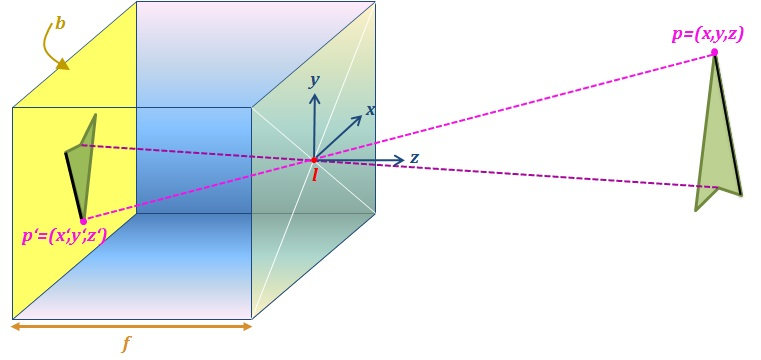
\includegraphics[width=8cm]{chapters/computervision/Grafik_1_Lochkamera.JPG}
\caption{Geometrie der Bildentstehung in einer Lochkamera.}
\label{fig:1}
\end{figure}
Eine Lochkamera ist eine schwarze Box, die an ihrer Front nur durch einen Punkt Licht eindringen lässt, welcher auf die Bildebene (Wand parallel zur Front) trifft. Je nachdem, wie gro"s die Lochblende ist, gelangen weniger oder mehr Lichtstrahlen hindurch. Je kleiner das Loch ist, desto schärfer ist das Bild, vor allem bei Objekten, die einen kleinen Abstand zur Lochkamera haben. Sobald das Loch vergrö"sert wird, gelangen mehr Lichtstrahlen hindurch, also wird ein Punkt vom Objekt durch mehrere Lichtstrahlen auf die Bildebene geschickt und das Bild erscheint uns unscharf.
\begin{figure} [h]
\centering
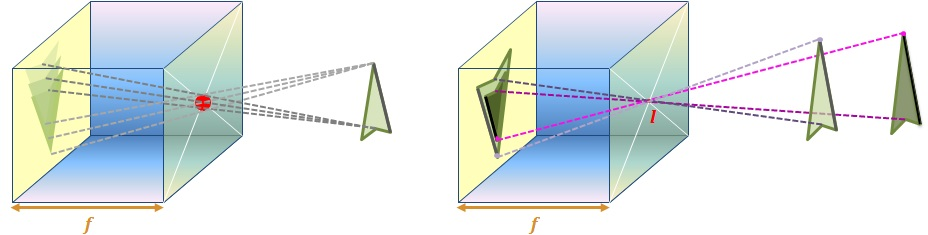
\includegraphics[width=12cm]{chapters/computervision/Grafik_3_Lochkamera.JPG}
\caption{Größe der Lochblende beeinflusst die Schärfe (links), der Abstand vor der Lochblende beeinflusst die Projektionsgrö"se (rechts).}
\label{fig:3}
\end{figure}

Wir betrachten einen Punkt $p$ mit den Koordination $(x,y,z)$ und seine \glqq Kopie\grqq\ $p'=(x',y',z')$ auf der Bildebene. $f$ beschreibt den Abstand zwischen der Lochblende $l$ und der Bildebene $b$.
\begin{figure}[h]
\centering
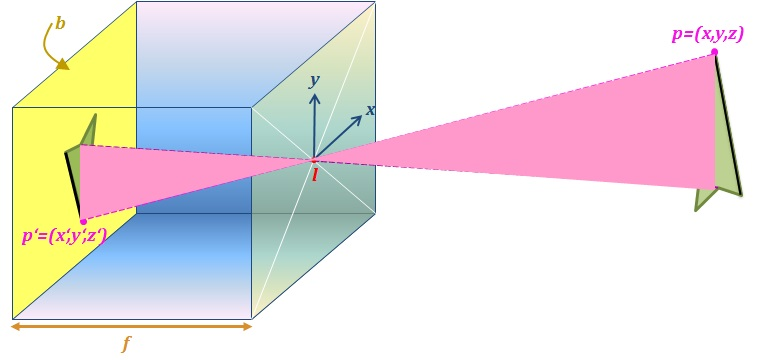
\includegraphics[width=8cm]{chapters/computervision/Grafik_2_Lochkamera.JPG}
\caption{Invertierte, gleiche Dreiecke.}
\label{fig:2}
\end{figure}
Es entstehen zwei kongruente Dreiecke, sodass wir die folgenden Umformungen vornehmen können:
\[\frac{-x'}{f}=\frac{x}{z},\quad \frac{-y'}{f}=\frac{y}{z} \quad \Rightarrow \quad x'=\frac{-fx}{z}, \quad y'=\frac{-fy}{z}\]
Wie auf der Abbildung zu sehen ist, wird das Objekt auf der Bildebene invertiert, sodass das Objekt sowohl auf dem Kopf steht als auch gespiegelt ist (in der Gleichung ist dieser Vorgang durch das negative Vorzeichen markiert). Was hier passiert hei"st \textbf{perspektivische Projektion}: parallele Linien treffen sich in einem \textbf{Fluchtpunkt} in der Ferne. Hierfür ist ausschlie"slich der Richtungsvektor der Linien ausschlaggebend.
Für eine Linie mit der Richtung $(u,v,w)$, die durch einen Punkt $p=(x,y,z)$ geht, gilt, dass die Projektion $P_\lambda$ auf der Bildebene für jeden Punkt $p'=(x+\lambda u,y+\lambda v,z+\lambda w)$ mit $\lambda\in (-\infty,+\infty)$ auf ihr durch
\[P_\lambda=\Bigg( f\frac{x+\lambda u}{z+\lambda w},f\frac{v+\lambda v}{z+\lambda w} \Bigg)\]
gegeben ist.

\subsubsection{Linsensysteme}
Linsen sind dem menschlichen Auge nachempfunden und im Vergleich zu Lochblenden viel grö"ser, sodass mehr Licht hindurch gelangt. Dadurch können nicht alle Objekte der Welt gleichzeitig scharf auf der Bildebene abgebildet werden, sondern nur solche, die sich im Bereich der \textbf{Tiefenschärfe} - also in einem bestimmten Abstand zur Linse - befinden.

In der Linse werden alle von einem Objekt eingehenden Strahlen so gebrochen, dass sie sich in einem Punkt hinter der Linse schneiden.
Die \textbf{Brennweite} $f$ der Linse, bei der ein bestimmtes Objekt scharf dargestellt wird, ergibt sich aus den Punkten $z$ (Abstand des Objekts zur Linse) und $z'$ (Abstand von der Linse zur Bildebene). Die Beziehung zwischen $z$ und $z'$ wird mit
\[\frac{1}{z}+\frac{1}{z'}=\frac{1}{f}\]
beschrieben. Da $z$ überwiegend sehr viel grö"ser als $z'$ ist, wird die Abschätzung
\[\frac{1}{z}+\frac{1}{z'}\approx\frac{1}{z'}\quad\Rightarrow\quad\frac{1}{z'}\approx\frac{1}{f}\quad\Rightarrow z'\approx f.\]
gemacht.

\subsubsection{Licht und Schatten}

Typischerweise wird die Bildebene in einer Kamera mit einem Pixel-Raster der Grö"se $512\times 512$ bemessen. Die Bildhelligkeit über die Zeit wird durch $I(x,y,t)$ repräsentiert und kann modelliert werden. Sie ist von der vorhandenen Lichtmenge, der Objekt-Position und der Reflexionseigenschaften während der Bildaufnahme abhängig, wobei die Oberfläche des Objektes als auch die umliegenden Objekte Reflexionseigenschaften besitzen.
\begin{itemize}
\item
Wir sprechen von diffus reflektiertem Licht, wenn das Licht von der Objektoberfl"ache absorbiert und wieder abgestrahlt wurde, wodurch die Oberfl"ache von allen Richtungen aus gleich hell erscheint. Eine \textit{Lambert'sche} Ebene oder \emph{perfekter Streuk"orper} ist ein Objekt, das Licht vollst"andig diffus reflektiert. Ein perfekter Streukörper erzeugt die reflektierte Lichtintensität
$E = p\cdot E_0\cdot \mathrm{cos}\theta$
mit Lichtquelle $E_0$, Rückstrahlvermögen $p\in\lbrack 0,1\rbrack$ (schwarz bis wei"se Ebene) und $\theta$ zwischen der Richtung der Lichtquelle und der Oberfl"achennormale.
\item
Das spiegelnd reflektierte Licht hingegen wird "uberwiegend in eine bestimmte Richtung abgestrahlt. Der Reflexionswinkel stimmt hierbei mit dem Einfallswinkel überein, wie bei einer \textit{perfekten Spiegelreflexion}.
\item
Durch Unterschiede in der Lichtintensität entstehen \textbf{Schatten} auf Objekt-Oberflächen. Aus der gegebenen Helligkeit $I(x,y)$ unseres Bildes möchten wir auf die Geometrie und Reflexionseigenschaften der Umwelt schlie"sen. Für Oberflächen von Objekten können wir eine Reflexionskarte berechnen, welche ihre Reflexionseigenschaften beschreibt.
\end{itemize}
Bei der Computergrafik wird genau diese Lichtsituation, also die Welt um das Objekt, wo Licht aus verschiedenen Richtungen kommt und (mehrfach) reflektiert wird, versucht zu simulieren.
Normalerweise ist eine Mischung von direktem und indirektem Licht vorhanden. Wenn solche Interreflexion vorliegt, hilft uns die Reflexionskarte nicht weiter - ein Problem, welches noch nicht gelöst ist.

\subsubsection{Spektralphotometrie}

Neben dem Kontrastsehen gibt es noch das Farbsehen, welches sich in einem Wellenlängenbereich von Violett bis Rot, $400$nm--$700$nm, bewegt. Das menschliche Auge ist für drei verschiedene Spektralkurven empfindsam, sodass der unendlich-dimensionale Bereich der Wellenlänge auf einen drei-dimensionalen Farbbereich projiziert wird. So kommt es zu sogenannten \textbf{Metameren}: Verschiedene Lichtspektren, die von Menschen als gleiche Farben wahrgenommen werden.

\section{Weitere Anwendungsgebiete}
Die Hauptanwendungsgebiete neben der \textbf{Objekterkennung} sind \textbf{Manipulation} der dreiminesionalen Welt und \textbf{Navigation} (Pfaderkennung, Ausweichmanöver, etc.). Diese und andere Einsatzgebiete neben den zur Veranschaulichung schon bereits besprochenen Nutzungsmöglichkeiten der Objekterkennung werden in den folgenden Abschnitten dargelegt.


\subsection{Bilder und Schlagworte}
Heutzutage bietet das Internet die Möglichkeit, anhand von Schlagwörtern nicht nur nach Text zu suchen, sondern auch Bilder zu finden. Das automatisierte Versehen von Bilder mit Schlagworten ist sehr wichtig: Wir haben eine Menge von Beispielbildern und möchten mit diesen einige Testbilder abgleichen (\textbf{Problem der Auto-Annotation}). Das beste Ergebnis erhält man mit der \textbf{Nächste-Nachbarn-Klassifikation}, die die Trainingsbilder raussucht, die dem Testbild durch bestimmte Merkmalsausprägungen am ähnlichsten sind. Die Schwierigkeit liegt in der Erkennung von Aktionsmustern. Man kann zwar schon durch Hintergrundsubtraktion und anschließeneder Betrachtung von HOG-Merkmalen basierend auf dem optischen Fluss die Verhaltensstrukturen annährend gut erkennen und so beispielsweise einen trinkenden Menschen im Bild ausfindig machen (Hand wird mit Objekt zum Mund geführt), allerdings ist diese Erkennung sehr eingeschränkt: Man könnte mit diesen Merkmalsausprägungen keine trinkende Katze in einem Bild erkennen.


\subsection{Rekonstruktion}
Besteht die Vermutung, was für ein Objekt sich auf einem Testbild befindet, so reicht manchmal allein schon dieses Bild aus, um mehrere Ansichten des Objekts zu erstellen. Wenn das Objektmodell, d.h. die Repräsentation des Objekts in dem Klassifizierer, aus mehreren Punkten oder sogar Bildern besteht, können wir Korrespondenzen zu Punkten aus dem Testbild dokumentieren. Anhand der Punkte können wir dann die Parameter der Kamera, falls diese nicht vorliegen, bestimmen und überprüfen, ob die Modellpunkte mit den Bildpunkten übereinstimmen.

Diese Technologie der Rekonstruktion ist heutzutage so hochentwickelt, dass sie in folgenden Bereichen zur Anwendung kommt:
\begin{itemize}
  \item \textbf{Modellerstellung} (z.B. dreidimensionale Karten)
  \item \textbf{Bewegungsabgleich} (z.B. bei animierte Figuren in realen Filmsequenzen)
  \item \textbf{Pfadrekonstruktion} (z.B. bei mobilen Robotern)
\end{itemize}


\subsection{Bewegungssteuerung}
Wie wichtig die Manipulation von Objekten und die Navigation beispielweise beim Ausweichen von Hindernissen ist, wird nicht nur in der Tierwelt deutlich. Wollen wir ein Visionssystem für ein \textbf{selbstfahrendes Fahrzeug} implementieren, so hat dies für folgende Aufgaben geeignete Aktionen zu finden:
\begin{itemize}
  \item \textbf{Seitensteuerung}: innerhalb der Spur bleiben oder Spurwechsel ausführen.
  \item \textbf{Längssteuerung}: bremsen, beschleunigen, Abstand halten.
  \item \textbf{Ausweichen}: Objekte in der Nähe beobachten und Kollisionen vermeiden.
\end{itemize}
Für die Seitensteuerung werden Algorithmen zur Kantenerkennung: Sie dienen dazu, Mittelstreifen zu erkennen und die Position und Ausrichtung des Autos relativ zur Spur zu verwalten.\\
Für die Längssteuerung und das Wahrnehmen von Hindernissen müssen wir Abstandserkennung mit Strukturerkennung kombinieren: Durch binokulares Stereosehen oder durch optischen Fluss, unterstützt durch HOG-Merkmale, können sich Fahrzeuge an Verkehrsregeln halten.

Mobile Roboter stellen eine größere Herausforderung da. Eine Methode zur Lokalisierung dieser in ihrer Umgebung besteht aus stereoskopischen Kamerasystemen. Um bei schlechten Lichtverhältnissen mit genügend Informationen versorgt zu werden, ist von den zwei Systemen eins nach vorne und das andere nach hinten ausgerichtet. Sollte die Beleuchtung allerdings doch mal erheblich schlecht sein, sorgt ein Trägheitsmodul, das ähnlich wie unser Gleichgewichtsorgan funktioniert, für die weitere Informationsbereitstellung.

Ein weiteres Problem der (visuellen) \textbf{Odometrie} (Bestimmung der Positionsänderung) ist die "`Drift"', bei der sich kleine Positionsabweichungen mit der Zeit aufaddieren. Zur Lösung dieses Problems werden feste Standpunkte in der Umgebung installiert, an denen der Roboter sich orientieren kann.
